\documentclass[conference]{IEEEtran}
\IEEEoverridecommandlockouts
% The preceding line is only needed to identify funding in the first footnote. If that is unneeded, please comment it out.
\usepackage{cite}
\usepackage{amsmath,amssymb,amsfonts}
\usepackage{algorithmic}
\usepackage{graphicx}
\usepackage{textcomp}
\usepackage{xcolor}
\usepackage[utf8]{inputenc} % Para que las tildes y ñ funcionen
\usepackage[T1]{fontenc}    % Mejor codificación de fuente
\usepackage[spanish]{babel} % ¡Este es el importante!
\def\BibTeX{{\rm B\kern-.05em{\sc i\kern-.025em b}\kern-.08em
    T\kern-.1667em\lower.7ex\hbox{E}\kern-.125emX}}
\begin{document}

\title{Título de la práctica de laboratorio\\}

\author{\IEEEauthorblockN{1\textsuperscript{ro} Apellidos Nombres}
\IEEEauthorblockA{\textit{Carrera} \\
\textit{Universidad Centroamericana (UCA)}\\
Antiguo Cuscatlán, El Salvador \\
Correo electrónico}
\and
\IEEEauthorblockN{2\textsuperscript{do} Apellidos Nombres}
\IEEEauthorblockA{\textit{Carrera} \\
\textit{Universidad Centroamericana (UCA)}\\
Antiguo Cuscatlán, El Salvador \\
Correo electrónico}
\and
\IEEEauthorblockN{3\textsuperscript{ro} Apellidos Nombres}
\IEEEauthorblockA{\textit{Carrera} \\
\textit{Universidad Centroamericana (UCA)}\\
Antiguo Cuscatlán, El Salvador \\
Correo electrónico}
\and
\IEEEauthorblockN{4\textsuperscript{to} Apellidos Nombres}
\IEEEauthorblockA{\textit{Carrera} \\
\textit{Universidad Centroamericana (UCA)}\\
Antiguo Cuscatlán, El Salvador \\
Correo electrónico}
\and
\IEEEauthorblockN{5\textsuperscript{to} Apellidos Nombres}
\IEEEauthorblockA{\textit{Carrera} \\
\textit{Universidad Centroamericana (UCA)}\\
Antiguo Cuscatlán, El Salvador \\
Correo electrónico}
\and
\IEEEauthorblockN{6\textsuperscript{to} Apellidos Nombres}
\IEEEauthorblockA{\textit{Carrera} \\
\textit{Universidad Centroamericana (UCA)}\\
Antiguo Cuscatlán, El Salvador \\
Correo electrónico}
}

\maketitle

\begin{abstract}
El resumen representación abreviada, precisa y concisa del contenido completo del documento. Debe de explicar qué se hizo, cómo se hizo , qué resultados se obtuvieron y qué significan estos resultados. Debe de consistir en un solo párrafo, no debe de contener citas bibliográficas ni referencias a imágenes o figuras. Debe de redactarse en pasado impersonal (se encontró, se observó) y no deben usarse siglas o abreviaturas, excepto las que todos conocen.
\end{abstract}

\begin{IEEEkeywords}
Máximo 7 palabras o frases cortas que tengan una relación directa con el tema tratado en el artículo
\end{IEEEkeywords}

\section{Introducción}
La introducción de este artículo científico tiene como propósito establecer el marco teórico fundamental para la comprensión del fenómeno físico en estudio. En esta sección, se exponen de manera articulada los conceptos teóricos esenciales derivados de las guías de laboratorio, acompañados de las ecuaciones matemáticas que rigen el comportamiento del sistema. Para facilitar la interpretación de estos conceptos abstractos, se integran diagramas e imágenes ilustrativas que vinculan la teoría con la realidad física. Cabe destacar que toda la información presentada ha sido rigurosamente obtenida de fuentes bibliográficas confiables, garantizando la integridad académica al prescindir de contenido generado por inteligencia artificial y priorizando el sustento científico de autores reconocidos.

\section{Metodología}

Constituye la descripción técnica y procedimental del experimento, redactada con un nivel de detalle que garantice la replicabilidad total de la práctica. En ella se deben enlistar de forma exhaustiva los materiales y equipos utilizados, especificando obligatoriamente la resolución e incertidumbre de los instrumentos críticos para establecer el margen de error experimental. El procedimiento debe narrarse de manera cronológica y minuciosa en pasado impersonal, indicando el número de repeticiones efectuadas en cada medición para sustentar la validez estadística de los datos. Finalmente, es indispensable integrar un diagrama o esquema del montaje experimental que ilustre la disposición y conexión de los componentes, sirviendo como guía visual para complementar la descripción textual de la configuración.

\begin{table}[h!]
\centering
\caption{Ejemplo de tabla}
\label{tab:densidad_incertezas}
\begin{tabular}{ccc}
\hline
\textbf{Volumen (ml)} & \textbf{Masa (g)} & \textbf{Densidad (g/ml)} \\ \hline
1.00 $\pm$ 0.05 & 0.995 $\pm$ 0.001 & 0.995 $\pm$ 0.05 \\
2.00 $\pm$ 0.05 & 2.063 $\pm$ 0.001 & 1.03 $\pm$ 0.03 \\
3.00 $\pm$ 0.05 & 3.047 $\pm$ 0.001 & 1.02 $\pm$ 0.02 \\
4.00 $\pm$ 0.05 & 4.059 $\pm$ 0.001 & 1.02 $\pm$ 0.01 \\
5.00 $\pm$ 0.05 & 5.013 $\pm$ 0.001 & 1.00 $\pm$ 0.01 \\
6.00 $\pm$ 0.05 & 6.032 $\pm$ 0.001 & 1.01 $\pm$ 0.01 \\
7.00 $\pm$ 0.05 & 7.019 $\pm$ 0.001 & 1.00 $\pm$ 0.01 \\
8.00 $\pm$ 0.05 & 7.990 $\pm$ 0.001 & 0.999 $\pm$ 0.006 \\
9.00 $\pm$ 0.05 & 8.953 $\pm$ 0.001 & 0.995 $\pm$ 0.006 \\
10.00 $\pm$ 0.05 & 9.944 $\pm$ 0.001 & 0.994 $\pm$ 0.005 \\
11.00 $\pm$ 0.05 & 10.928 $\pm$ 0.001 & 0.993 $\pm$ 0.005 \\
12.00 $\pm$ 0.05 & 11.993 $\pm$ 0.001 & 0.999 $\pm$ 0.004 \\ \hline
\end{tabular}
\end{table}

\begin{figure}[htbp]
\centerline{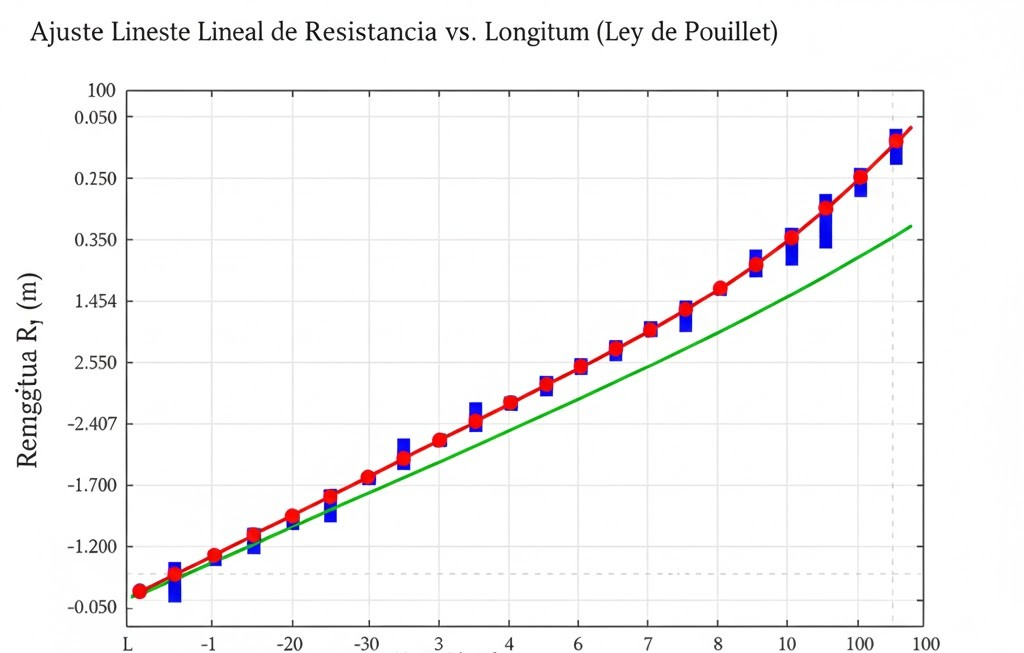
\includegraphics[scale=0.3]{unnamed.jpg}} % Reduce al 40% del tamaño original
\caption{Ejemplo de gráfico}
\label{fig}
\end{figure}


\section{Análisis y discusión}
\subsection{Análisis}
La sección de análisis comienza con la presentación sistemática de los datos experimentales, los cuales deben seguir estrictamente el convenio de cifras significativas e incertidumbres para garantizar su validez técnica. Para facilitar la comprensión del fenómeno, se debe integrar una representación gráfica de las variables, sobre la cual se aplicará un ajuste por mínimos cuadrados que permita identificar la tendencia funcional del modelo. Es imperativo que el estudiante realice una interpretación física de los coeficientes obtenidos (como la pendiente y el intercepto), vinculándolos directamente con las leyes teóricas descritas en la introducción. Se debe explicar de forma coherente si los hallazgos personales validan o refutan la hipótesis inicial, contrastando estos valores con patrones reportados en fuentes bibliográficas confiables. Finalmente, el análisis debe culminar en una evaluación crítica que determine qué objetivos se cumplieron y cuáles factores de error afectaron el experimento, proponiendo mejoras metodológicas concretas que sirvan de base para las conclusiones finales del artículo.
\subsection{Discusión}
La discusión de los resultados permite interpretar el significado de los datos obtenidos, evaluando directamente cómo responden a las hipótesis y objetivos planteados al inicio de la investigación. En este apartado, es fundamental vincular los hallazgos con la teoría y los conceptos fundamentales que sirven de base para el artículo, demostrando la congruencia o divergencia entre la observación experimental y el modelo físico establecido. Se deben analizar las implicaciones prácticas y teóricas de los resultados, destacando su relevancia en el contexto del estudio de los fenómenos físicos. Asimismo, es imperativo reconocer las limitaciones del estudio, tales como el alcance de los instrumentos o factores ambientales, para contextualizar los hallazgos y evitar generalizaciones excesivas que no estén soportadas por la evidencia. Finalmente, a partir de la experiencia adquirida, se deben proponer nuevos métodos prácticos o modificaciones en el diseño experimental que puedan refinar futuras investigaciones y optimizar la obtención de datos.

\section{Conclusiones}

Las conclusiones sintetizan el estudio reiterando el propósito inicial del experimento para verificar el cumplimiento de los objetivos planteados. En este apartado se presentan de forma concisa los resultados y descubrimientos más significativos, permitiendo declarar con fundamento estadístico si la hipótesis fue aceptada o rechazada según la evidencia recolectada. Es fundamental ofrecer una explicación lógica de por qué se obtuvieron dichos resultados, interpretando su significado físico y discutiendo las consecuencias e impacto de estos hallazgos en el área de estudio. Asimismo, se debe realizar una evaluación crítica sobre la fiabilidad del experimento, exponiendo con honestidad las dificultades técnicas o limitaciones que pudieron sesgar los datos. Finalmente, el texto debe proyectarse hacia el futuro, proponiendo mejoras específicas y nuevas líneas de acción que podrían abordarse para optimizar la precisión y el alcance de investigaciones posteriores.

\section*{Normas de Citación y Referencias}

La plantilla numerará las citas de forma consecutiva entre corchetes [1]. La puntuación de la oración sigue al corchete [2]. Remítase simplemente al número de referencia, como en [3]—no utilice ``Ref. [3]'' ni ``referencia [3]'' excepto al principio de una oración: ``La referencia [3] fue la primera ...''.

Numere las notas al pie por separado mediante superíndices. Coloque la nota al pie real en la parte inferior de la columna en la que fue citada. No incluya notas al pie en el resumen ni en la lista de referencias. Utilice letras para las notas al pie de las tablas.

A menos que haya seis autores o más, indique los nombres de todos los autores; no utilice ``et al.''. Los artículos que no hayan sido publicados, incluso si han sido enviados para su publicación, deben citarse como ``inéditos'' [4]. Los artículos que hayan sido aceptados para su publicación deben citarse como ``en prensa'' [5]. Escriba con mayúscula solo la primera palabra del título de un artículo, excepto para nombres propios y símbolos de elementos.

\begin{thebibliography}{00}
\bibitem{b1} G. Eason, B. Noble, and I. N. Sneddon, ``On certain integrals of Lipschitz-Hankel type involving products of Bessel functions,'' Phil. Trans. Roy. Soc. London, vol. A247, pp. 529--551, April 1955.
\bibitem{b2} J. Clerk Maxwell, A Treatise on Electricity and Magnetism, 3rd ed., vol. 2. Oxford: Clarendon, 1892, pp.68--73.
\bibitem{b3} I. S. Jacobs and C. P. Bean, ``Fine particles, thin films and exchange anisotropy,'' in Magnetism, vol. III, G. T. Rado and H. Suhl, Eds. New York: Academic, 1963, pp. 271--350.
\bibitem{b4} K. Elissa, ``Title of paper if known,'' unpublished.
\bibitem{b5} R. Nicole, ``Title of paper with only first word capitalized,'' J. Name Stand. Abbrev., in press.
\bibitem{b6} Y. Yorozu, M. Hirano, K. Oka, and Y. Tagawa, ``Electron spectroscopy studies on magneto-optical media and plastic substrate interface,'' IEEE Transl. J. Magn. Japan, vol. 2, pp. 740--741, August 1987 [Digests 9th Annual Conf. Magnetics Japan, p. 301, 1982].
\bibitem{b7} M. Young, The Technical Writer's Handbook. Mill Valley, CA: University Science, 1989.
\end{thebibliography}
\end{document}
